\documentclass[11pt]{article}
\usepackage[utf8]{inputenc}
\usepackage[slovene]{babel}


\usepackage{lmodern}
\usepackage{hyperref}
\usepackage{blindtext}
\usepackage{amssymb}  
\usepackage{listings} %python koda
\usepackage{tabularx}
\usepackage{tikz}

\usepackage{amsthm}
\usepackage{amsmath, amssymb, amsfonts}
\usepackage{relsize}
\usepackage{graphicx}
\graphicspath{ {./Slike/} }
\usepackage{subcaption} % za side-by-side slike
\usepackage[
top    = 3.cm,
bottom = 3.cm,
left   = 3.cm,
right  = 3.cm]{geometry}
\usepackage{xcolor}

\newtheorem{definicija}{Definicija}[section]

\theoremstyle{definition}
\newtheorem*{navodilo}{Navodilo}
\newtheorem*{razmislek}{Razmislek}

\newtheorem{opomba}{Opomba}

\newcommand{\R}{\mathbb{R}}
\newcommand{\N}{\mathbb{N}}
\newcommand{\Z}{\mathbb{Z}}
\newcommand{\p}{\mathbb{P}}
\newcommand{\E}{\mathbb{E}}
\newcommand{\1}{\mathbbm{1}}
\newcommand{\set}[1]{\{#1\}}
\newcommand{\green}[1]{\color{teal}#1\color{black}}
\newcommand{\B}{\mathcal{B}}

\lstset{%
   breaklines=true
}

\begin{document}

\begin{titlepage} 

	\center 
	
	\textsc{\LARGE Univerza v Ljubljani}\\[0.5cm] 
	{\Large Fakulteta za matematiko in fiziko}\\[3cm] 
	
	{\large Finančni praktikum}\\[1.0cm]
	
	{\huge \textsc{Skoraj konstantne vsote trikotnih funkcij na zaprtem intervalu}}\\[1.0cm]
	
	{\large Poročilo}\\[3.0cm]
	
	\begin{minipage}{0.4\textwidth}
		\begin{flushleft}
			\large
			\textit{Avtorja:}\\
			Neža \textsc{Kržan} \\
			Oskar \textsc{Vavtar} 
		\end{flushleft}
	\end{minipage}
	~
	\begin{minipage}{0.4\textwidth}
		\begin{flushright}
			\large
			\textit{Mentorja:}\\
			prof. dr. Sergio \textsc{Cabello} \\
			doc. dr. Janoš \textsc{Vidali}
		\end{flushright}
	\end{minipage}
	
	\vfill\vfill\vfill 
	
	{\large{Ljubljana, \today}} 
	 
	\vfill 
	
\end{titlepage}

% #################################################################################################
\tableofcontents
\newpage

% #################################################################################################

\section{Uvod}
\vspace{0.5cm}

V poročilu bova predstavila problem izračuna skoraj konstantne vsote trikotnih funkcij na zaprtem intervalu in kodo, s katero sva problem rešila. 
V začetku poročila sledi podroben opis problema ter ugotovitve glede njegovega reševanja. V nadaljevanu sledijo komentrji na kodo in predstavitev rezultatov.

% #################################################################################################

\section{Navodilo}
\vspace{0.5cm}

Imamo nabor $n$ trikotnih funkcij. Izmed njih želimo izbrati podmnožico največ sedmih, da bo njihova vsota čim bolj konstantna na intervalu $[0,1]$ - s tem mislimo, da je razlika med maksimalno in minimalno vrednostjo vsote najmanjša možna. Ali je metoda celoštevilskega linearnega programiranja primerna za ta problem? Lahko uporabimo kakšne druge metode? Kako bi sami generirali smiselne vhodne podatke za ta problem? Bi lahko na enak način obravnavali tudi druge funkcije, npr. preproste stopničaste funkcije?

% *************************************************************************************************

\subsection{Razmislek in potek dela}
\vspace{0.5cm}

Očitno je, da je več aspektov tega problema mogoče posplošiti. Trikotne funkcije lahko nadomestimo s katerimi drugimi preprostimi funkcijami (npr. stopničastimi, pravokotnimi). Namesto 7 funkcij, jih lahko izberemo $r$, $r < n$. Namesto intervala $[0,1]$ pa lahko izberemo poljuben zaprt interval $[a,b]$, $-\infty < a \leq b < \infty$. \\

Problem sva se odločila rešiti za dva tipa trikotnih funkcij:
\begin{itemize}
	\item simetrične,
	\item splošne.
\end{itemize}

Problem sva nameravala reševati z metodo celoštevilskega linearnega programiranja, ki se je kasneje izkazala za neustrezno. Namesto tega sva uporabila metodo mešano-celoštevilskega programiranja, ki v dovoli tudi realnoštevilske omejitve. \\

Kot opisano v navodilu je ``čim bolj konstantno'' mišljeno kot čim manjša razlika med maksimalno in minimalno vrednostjo vsote funkcij na intervalu. Iz nabora funkcij $\set{f_1,\ldots,f_n}$ želimo torej izbrat tako podmnožico $\set{g_1,\ldots,g_r}$, $r \leq n$, da bo dosežen
$$\min_{\set{g_1,\ldots,g_r} \subseteq \set{f_1,\ldots,f_n}}\left({\max_{x \in [a,b]}\sum_{i=1}^r g_i - \min_{x \in [a,b]}\sum_{i=1}^r g_i}\right)$$
na želenem zaprtem intervalu $[a,b]$ (v navodilih $[a,b]=[0,1]$, $r=7$). Očitno je, da zgoraj zapisano ne formulira linearnega programa -- funkciji $\max$ in $\max$ nista linearni. Formulacijo je bilo zato potrebno še malo spremeniti. Pri tem sva si pomagala z dejstvom, da so trikotne funkcije, s katerimi imava opravka, odsekoma linearne -- ekstreme lahko dosežejo le v točkah, kjer se prelomijo. Ta lastnost se zaradi linearnosti prenese tudi na njihovo vsoto. Ta lahko ekstreme doseže le v točkah, kjer se prelomi neka funkcija, ki je del te vsote. 

% *************************************************************************************************

\subsection{Programsko okolje in implementacija}
\vspace{0.5cm}

Za implementacijo problema sva se odločila za uporabo programskega jezika \texttt{Sage}, ker ima že vgrajeno podporo za celoštevilsko linearno programiranje. V osnovi sloni na programskem jeziku \texttt{Python}, z dodatno podporo za matematiko, nastal pa je kot alternativa programskemu jeziku \texttt{Mathematica}. Programirala sva na platformi \texttt{CoCalc}, kjer sva datoteke pretvorila v \texttt{Jupyter Notebooks} obliko. Za prikaz rezultatov pri eksperimentiranju sva uporabila \texttt{R}.

%#################################################################################################

\section{Ideja rešitve z linearnim programiranjem LP}
\vspace{0.5cm}

Kot omenjeno v uvodu, je ideja naslednja: iz nabora funkcij $\set{f_1,\ldots,f_r}$ želimo torej izbrati tako podmnožico $\set{g_1,\ldots,g_r}$, $r \leq 7 < n$, da bo dosežen
$$\min_{\set{g_1,\ldots,g_7} \subseteq \set{f_1,\ldots,f_n}}\left({\max_{x \in [a,b]}\sum_{i=1}^r g_i - \min_{x \in [a,b]}\sum_{i=1}^r g_i}\right)$$
na želenem zaprtem intervalu $[a,b]$. Glede na to, da imamo opravka s trikotnimi funkcijami, ki so odsekoma linearne, pa lahko problem poenostavimo. Iz odsekoma linearnosti tako funkcij kot njihove vsote sledi, da bo vsota lahko dosegla ekstrem le na robovih intervala ali na mestu prelomu ene izmed funkcij. Vsoto lahko zato namesto na celotnem intervalu $[a,b]$ ocenimo le na točkah preloma. Definiramo torej množico testnih točk $\mathcal{B} = \set{x_1,\ldots,x_k}$, v kateri so vsebovane točke preloma obravnavanih funkcij iz intervala $[a,b]$ ter robni točki $\set{a}$ in $\set{b}$. Da lahko v teh točkah ocenimo vsoto, moramo izračunati vrednosti vseh funkcij $f_j$, $j \in [n]$, v vseh točkah množice $\B$. Zgornjo formulacijo problema lahko prepišemo kot
$$\min \left( \max_{x_i \in \B} \sum_{j=1}^n f_j(x_i)v_j - \min_{x_i \in \mathcal{B}} \sum_{j=1}^n f_j(x_i)v_j \right),$$
kjer $v_j$ definiramo kot
$$v_j ~=~ \begin{cases}
1\,; ~&f_j \in \set{g_1,\ldots,g_r}, \\
0\,; ~&f_j \notin \set{g_1,\ldots,g_r}.
\end{cases}$$
Zdaj se moramo znebiti še funkcij $\max$ in $\min$. Izračunamo lahko vrednost $\sum_{j=1}^n f_j(x_i)v_j$ za vsak $i$ in definiramo vrednosti $M,m \in \R$, taki, da $M$ navzgor omeji dane vsote, $m$ pa navzdol.\\

Zdaj lahko zapišemo sledeč linearni program:
\begin{align*}
&\min(M-m) \\
&\forall j \in \set{1,\ldots,n}: ~0 \leq v_j \leq 1, ~v_j \in \Z \\
&\forall i \in \set{1,\ldots,k}: ~\sum_{j=1}^n f_j(x_i)v_j \leq M \\
&\forall i \in \set{1,\ldots,k}: ~\sum_{j=1}^n f_j(x_i)v_j \geq m \\
&\sum_{j=1}^n v_j \geq 1 \\
&\sum_{j=1}^n v_j \leq 7
\end{align*}
Ker sta $M$ in $m$ realnoštevilski omejitvi, ta linearen program ni celoštevilski ampak mešano-celoštevilski (MCLP).

% #################################################################################################

\section{Implementacija}
\vspace{0.5cm}

% *************************************************************************************************

\subsection{Generiranje trikotnih funkcij}
\vspace{0.5cm}

Definicija trikotne funkcije ni pretirano striktno določena, ideja pa je naslednja. 
Funkcija je konstantno enaka $0$ na intervalu $(-\infty, x_1)$, kjer $x_1$ predstavlja levi rob trikotnika. 
Na intervalu $[x_1, x_2]$, kjer je $(x_2,y(x_2))$ vrh trikotnika, je definirana kot linearna funkcija s pozitivnim naklonom, ki potuje skozi točki $(x_1,0)$ ter $(x_2,y(x_2))$. 
Na intervalu od $x_2$ do $x_3$, kjer je $x_3$ desni rob trikotnika, je zopet definirana kot linearna funkcija, tokrat z negativnim naklonom ter potuje skozi $(x_2,y(x_2))$ in $(x_3,0)$. 
Na intervalu $(x_3,\infty)$ je zopet konstantno enaka $0$. Najbolj preprost primer bi bil morda $f(x) = \max\set{1-|x|,0}$. \\

Pri samem generiranju trikotnih funkcij sva se odločila izkoristiti kar najin izbran način spopadanja s linearnim programom, pri katerem funkcijo oceniva le v končnem naboru točk preloma. Zato sva se odločila, da bova funkcije definirala preko njihovih točk preloma. Ideja je preposta: za dobljeno trojico točk $(x_1, 0),(x_2, y_2),(x_3,0) \in \R^2$, $x_1,x_2,x_3,y_1 \in \R$, \hbox{$x_1<x_2<x_3$, $y_2>0$,} lahko trikotno funkcijo $f$ definiramo kot
$$f(x) ~=~ \begin{cases}
0\,; ~&x \in (-\infty,x_1)\cup[x_3,\infty), \\
\frac{y_2}{x_2-x_1}x - \frac{y_2x_1}{x_2-x_1}\,; ~& x \in [x_1,x_2), \\
\frac{-y_2}{x_3-x_2}x + \frac{y_2x_3}{x_3-x_2}\,; ~& x \in [x_2, x_3).
\end{cases}$$
Točke sva generirala naključno, s pomočjo \texttt{Python}-ove knjižnice \texttt{random}. Definirala sva razred \texttt{TrikotnaFunkcija}, ki generira vrednosti po enakomerni zvezni porazdelitvi, 
\begin{align*}
x_1,x_2,x_3 ~&\sim~ \mathcal{U}([-2,2]), \\
y_2 ~&\sim~ \mathcal{U}([-10,10]), 
\end{align*}
ter jih nato uredi v točke $(x_1,0),(x_2,y_2),(x_3,0)$.

% *************************************************************************************************
\subsection{Koda za MCLP}
\vspace{0.5cm}

S pomočjo spodnje kode sva reševala linearni program. 
Funkcija \texttt{vsota\char`_trikotnih\char`_funkcij} reši MCLP. Omenjena funkcija vrne minimalno razliko med $M$ in $m$, ter trikotne funkcije, izbrane za izračun čim bolj konstantne vsote.

\begin{verbatim}
def vsota_trikotnih_funkcij(seznam_funkcij, seznam_tock, z):
    k = len(seznam_tock)
    r = len(seznam_funkcij)

    p = MixedIntegerLinearProgram(maximization=False)
    v = p.new_variable(binary=True)
    m = p.new_variable(integer=False, nonnegative=True)
    p.set_objective(m[1]-m[0])

    for x in seznam_tock:
        sum_ = sum(seznam_funkcij[j](x) * v[j] for j in range(r))
        f'{sum_=}'
        f'{sum_ - m[1]}'
        f'{sum_ - m[0]}'
        p.add_constraint(sum_ - m[1], max=0)
        p.add_constraint(sum_ - m[0], min=0)


    sum2_ = sum(v[j] for j in range(z))
    f'{sum2_=}'
    f'{v[0]=}'
    f'{z=}'
    p.add_constraint(sum2_, min=1)
    p.add_constraint(sum2_, max=z)

    vsota = p.solve()
    M, m = p.get_values(m[1]), p.get_values(m[0])
    f'{M=}'
    f'{m=}'
    v_resitve = p.get_values(v)
    f'{p.get_values(v)}'

    vkljucene_funkcije = [seznam_funkcij[j] for j in v_resitve if v_resitve[j]==1]

    return [vsota, vkljucene_funkcije]
\end{verbatim}

% *************************************************************************************************

% #################################################################################################

\section{Ugotovitve}
\vspace{0.5cm}

% *************************************************************************************************

\subsection{Eksperimentiranje}
\vspace{0.5cm}

Odločila sva se za generiranje programa tako, da sva spreminjala nabor trikotnih funckij (oz. prilagajala število $n$) na intervalu $[0,1]$. Zanimalo naju je kako konstantna je vosta oziroma kako se spremenja glede na večanje števila $n$. Predvidevala sva, da večji kot bo $n$ bolj konstantna bo vsota. Odločila sva se, da za vsak $n$ funkcijo \texttt{vsota\char`_trikotnih\char`_funkcij} zaženeva desetkrat, saj se nama je to zdelo dovolj. 
Zanimalo naju je tudi, kako program izbira funckije iz nabora $n$ trikotnih funkcij. Predvidevala sva, da manjše kot bo število $n$, manjša je verjetnost, da bo izbral večje število trikotnih funkcij za izračun čim bolj konstantne vsote na intervalu $[0,1]$. \\
\vspace{0.25cm}

Funckijo \texttt{vsota\char`_trikotnih\char`_funkcij} sva torej za vsak $n$ iz nabora $n = {7, 10, 25, 50, 80, 100}$ pognala desetkrat. Dobljeno število funkcij za izračun skoraj konstantne vsote trikotnih funkcij na zaprtem itervalu $[0,1]$ sva zapisovala v seznam in prav tako vsoto. 
Ugotovila sva, kar je razvidno tudi iz spodnjega grafa (a)Í, da večje kot je število $n$ bolj konstantna je vsota. Večje kot je bilo število $n$, dlje časa je tudi program porabil za izračun. \\

Glede na število trikotnih funkcij, ki jih program izbere iz nabora $n$ trikotnih funkcij, sva prišla do ugotovitve, da večje kot je število $n$, več funkcij je program izbral za izračun, kar je vidno tudi na spodnjem grafu (b). \\	

\begin{figure}[h!]
\begin{center}
	\begin{subfigure}{0.5\textwidth}
	\begin{center}
		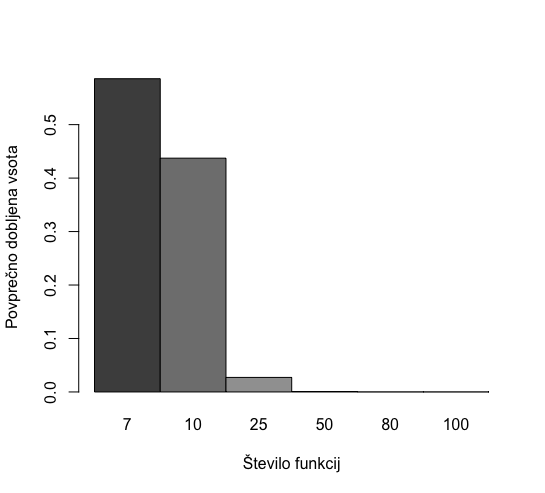
\includegraphics[width=0.98\textwidth]{vsota.png}
		\subcaption{Skoraj konstantne vsote trikotnih funkcij na \\zaprtem intervalu}
\end{center}
	\end{subfigure}%
	\begin{subfigure}{0.5\textwidth}
	\begin{center}
		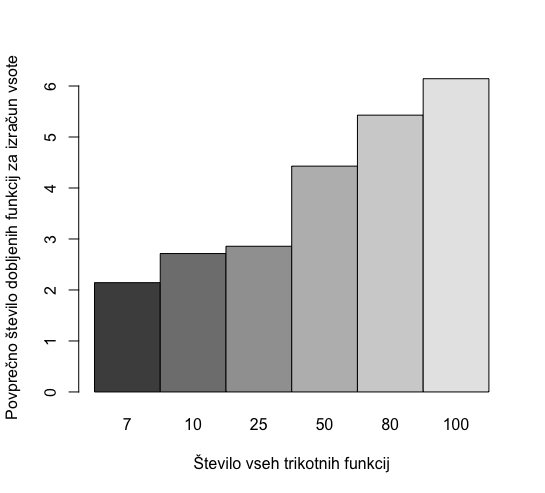
\includegraphics[width=0.98\textwidth]{st_funkcij.png}
		\subcaption{Število izbranih trikotnih funkcij glede na nabor vseh trikotnih funkcij} 
\end{center}
	\end{subfigure}
\end{center}
\end{figure}

\newpage
Še vedno so se pojavili primeri, ko je program izbral po le eno funkcijo iz nabora. 
Ugotovila sva tudi, da če je bila vsota enaka $0.00$, je program ponavaid izbral po eno ali dve funkciji iz nabora $n$ funkcij (seveda je bilo nekaj izjem).\\

% *************************************************************************************************
\subsection{Čas izvajanja programa}
\vspace{0.5cm}

Spodnji graf nam prikazuje, kako se povprečno spreminja čas izvajanja programa, ki je mešano - celoštevilski, za iskanje največ $7$ trikotnih funkcij v odvisnosti od celotnega nabora trikonih funkcij. 
Funckijo \texttt{vsota\char`_trikotnih\char`_funkcij} sva pognala za izbor največ $7$ trikotnih funkcij izmed $n$ trikotnih funkcij, kjer je $n = {7, 10, 25, 50, 60, 70}$.
Iz grafa sva razbrala, da se seveda čas izvajanja poveča s povečanjem nabora vseh trikotnih funkcij, kar je precej očitno. Program mora za vsako funkcijo več izračunati vse potrebne vsote in vsako funkcijo izračunati v naboru točk preloma. \\

\begin{figure}[h!]
	\centering
	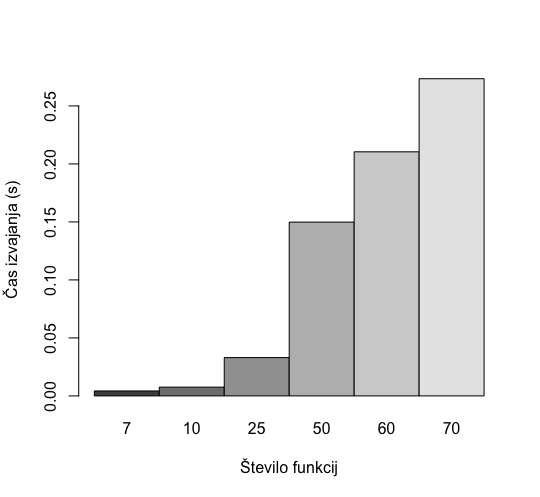
\includegraphics[scale=0.55]{casi.png}
	\caption{Čas izvajanja programa glede na spreminjanje celotnega nabora trikotnih funkcij}
\end{figure}

\pagebreak

% *************************************************************************************************

% #################################################################################################
\vspace{0.5cm}

\section*{Viri}
\vspace{0.5cm}
\begin{itemize}
	\item[{[1]}] Arjana Žitnik (2021). Prosojnice Celoštevilsko linearno programiranje, časovna zahtevnost in težki problemi.
		Dostopno \href{https://ucilnica2021.fmf.uni-lj.si/pluginfile.php/58787/mod_resource/content/13/CLP.pdf}{\color{blue}\underline{tukaj}\color{black}}.
	\item[{[2]}] Posvetovanje z asistentom Janošom Vidalijem in s profesorjem Sergiom Cabellom.
	\item[{[3]}] \texttt{http://fe.math.kobe-u.ac.jp}. Mixed integer linear programming. Dostopno \href{http://fe.math.kobe-u.ac.jp/icms2010-dvd/SAGE/www.sagemath.org/doc/reference/sage/numerical/mip.html}{\color{blue}\underline{tukaj}\color{black}}.
\end{itemize}

\end{document}